\documentclass{beamer} 
\usepackage{beamerthemeTUM}
\usepackage[latin1]{inputenc} 
\usepackage{amsmath} 
\usepackage{amsfonts} 
\usepackage{amssymb} 
\usepackage{algorithm} 
\usepackage{algorithmicx} 
\usepackage[noend]{algpseudocode}
\usepackage{multicol} 
\usepackage{url}
\usepackage{graphics}
\usepackage{multicol}
\usepackage{eso-pic}
\usepackage{pst-node}
\usepackage{xcolor}
\usepackage{multido}
\usepackage{subfigure}
\usepackage{pstricks}
\usepackage{float} 

\graphicspath{{figures/}}

\setlang{en}


\author{Sebastian Lehnerer} 
\title{Multilabel Attribute Selection} 

\subtitle{naive merging}
\email{lehnerer@in.tum.de}
\date{\today}
\institute[2011]{Technische Universit\"at M\"unchen}


\begin{document} 


\AddToShipoutPicture{\TitlePicture}
\maketitle
%\frame{\titlepage}
\ClearShipoutPicture
\AddToShipoutPicture{\BackgroundPicture}
\AtBeginPart{\frame{\partpage}}

\frame{
 {\insertsection} 
 \begin{itemize} 
  \item feature selection for every label, where other labels are
    treated as normal features
    \end{itemize} 
    \begin{eqnarray*} 
      Y_{1} &\leftarrow & \{X_{1}...X_{n} \cup Y_{2}...Y_{n}|X_{i},Y_{i}\in\{0,1\}\}\\ 
      Y_{2} &\leftarrow & \{X_{1}...X_{n} \cup Y_{1},Y_{3}...Y_{n}|X_{i},Y_{i}\in\{0,1\}\}\\ 
      &\vdots &\\ 
      Y_{n} &\leftarrow & \{X_{1}...X_{n} \cup Y_{1}...Y_{n-1}|X_{i},Y_{i}\in\{0,1\}\} 
    \end{eqnarray*} 
  
}

\frame{
	{\insertsection} 
	\begin{itemize}            
		\item  for every label, other label attributes in the corresponding feature set will be replaced by its feature set, until no labels remain the feature set. The elimited label are stored in a labelset which results in a map between label set and feature set  
		\item
		\begin{scriptsize}
		\begin{algorithmic}
		   \Function{findLabelFeatureSets}{data}
			   	\State $ groups \gets Map<labelSet, featureSet> $
		   		\For{$ L \in labelSet(data) $}
		    		\If{ $ L \notin keys(groups) $ }
			    		\State $ currentLabelSet \gets \{ L \} $
			    		\State $ currentFeatureSet \gets selectFeatures(L, data) $
			    		\While{ $ \exists \,\{ F \in currentFeatureSet \wedge F \in labelSet(data) \} $}
			    				\State $ currentLabelSet \cap \{F\} $
			    				\State $ currentFeatureSet \cap \{selectFeatures(F, data)\} $
			    				\State $ remove(F, currentFeatureSet) $
			    		\EndWhile
			    	\EndIf
		    	\EndFor
		    	\Return $groups$
		    \EndFunction
		  \end{algorithmic}
		\end{scriptsize}
	\end{itemize}  
}

\frame{
	{\insertsection} 
	\begin{itemize}            
		\item to avoid similiar label or feature-sets a second-step merge function is applied
		\item
		\begin{tiny}
		\begin{algorithmic}
		   \Function{backtrace}{groups}
		   		\For{$ labelSet \in keys(groups) $}
		   			\For{ $ labelSet2 \in keys(groups) $}
		   				\If{ $ labelSet2 \subset labelSet $}
		   					\State $ featureSet \gets groups(labelSet) $
		   					\State $ featureSet2 \gets groups(labelSet2) $
		   					\State $ groups(labelSet) \gets featureSet \cap featureSet2 $
		   					\State $ remove(labelSet2, groups) $
		   				\ElsIf{$ labelSet \subset labelSet2 $}
		   					\State $ featureSet \gets groups(labelSet) $
		   					\State $ featureSet2 \gets groups(labelSet2) $
		   					\State $ groups(labelSet2) \gets featureSet \cap featureSet2 $
		   					\State $ remove(labelSet, groups) $
		   				\ElsIf{$ groups(labelSet) \subset groups(labelSet2) $}
		   					\State $ groups(labelSet \cap labelSet2) \gets groups(labelSet2)  $
		   					\State $ remove(labelSet, groups) $
		   					\State $ remove(labelSet2, groups) $
						\ElsIf{$ groups(labelSet2) \subset groups(labelSet) $}
		   					\State $ groups(labelSet \cap labelSet2) \gets groups(labelSet)  $
		   					\State $ remove(labelSet, groups) $
		   					\State $ remove(labelSet2, groups) $
		   				\EndIf
		   			\EndFor
		   		\EndFor
		    	\Return $groups$
		    \EndFunction
		  \end{algorithmic}
		\end{tiny}
	\end{itemize} 
}

\frame{
 {\insertsection} 
		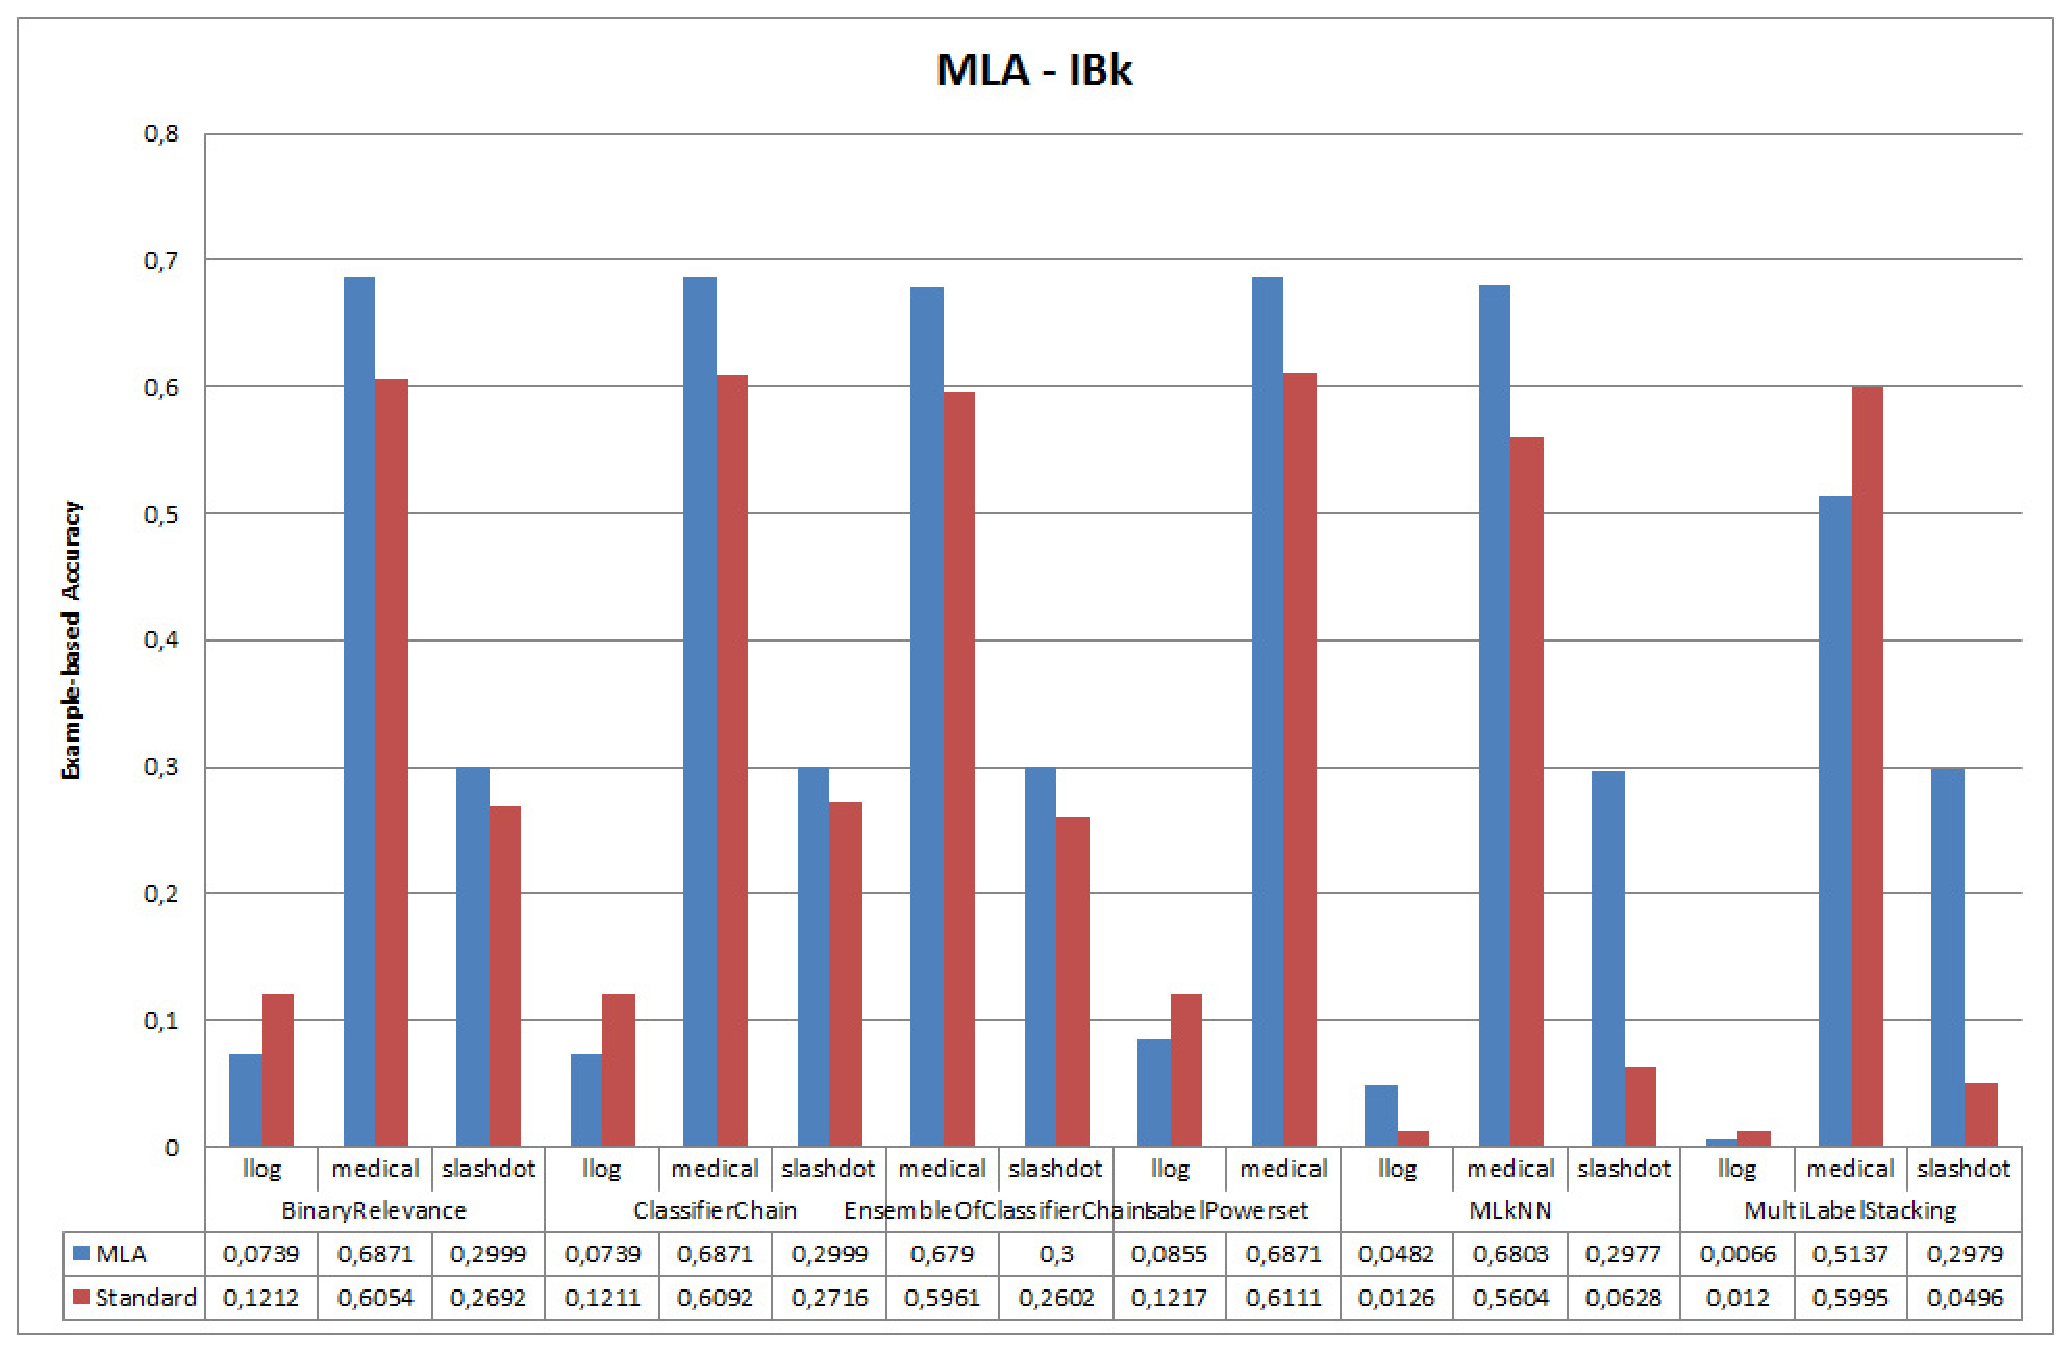
\includegraphics[scale=.3]{figures/mla_results_ibk.eps} 
}


\frame{
 {\insertsection} 
		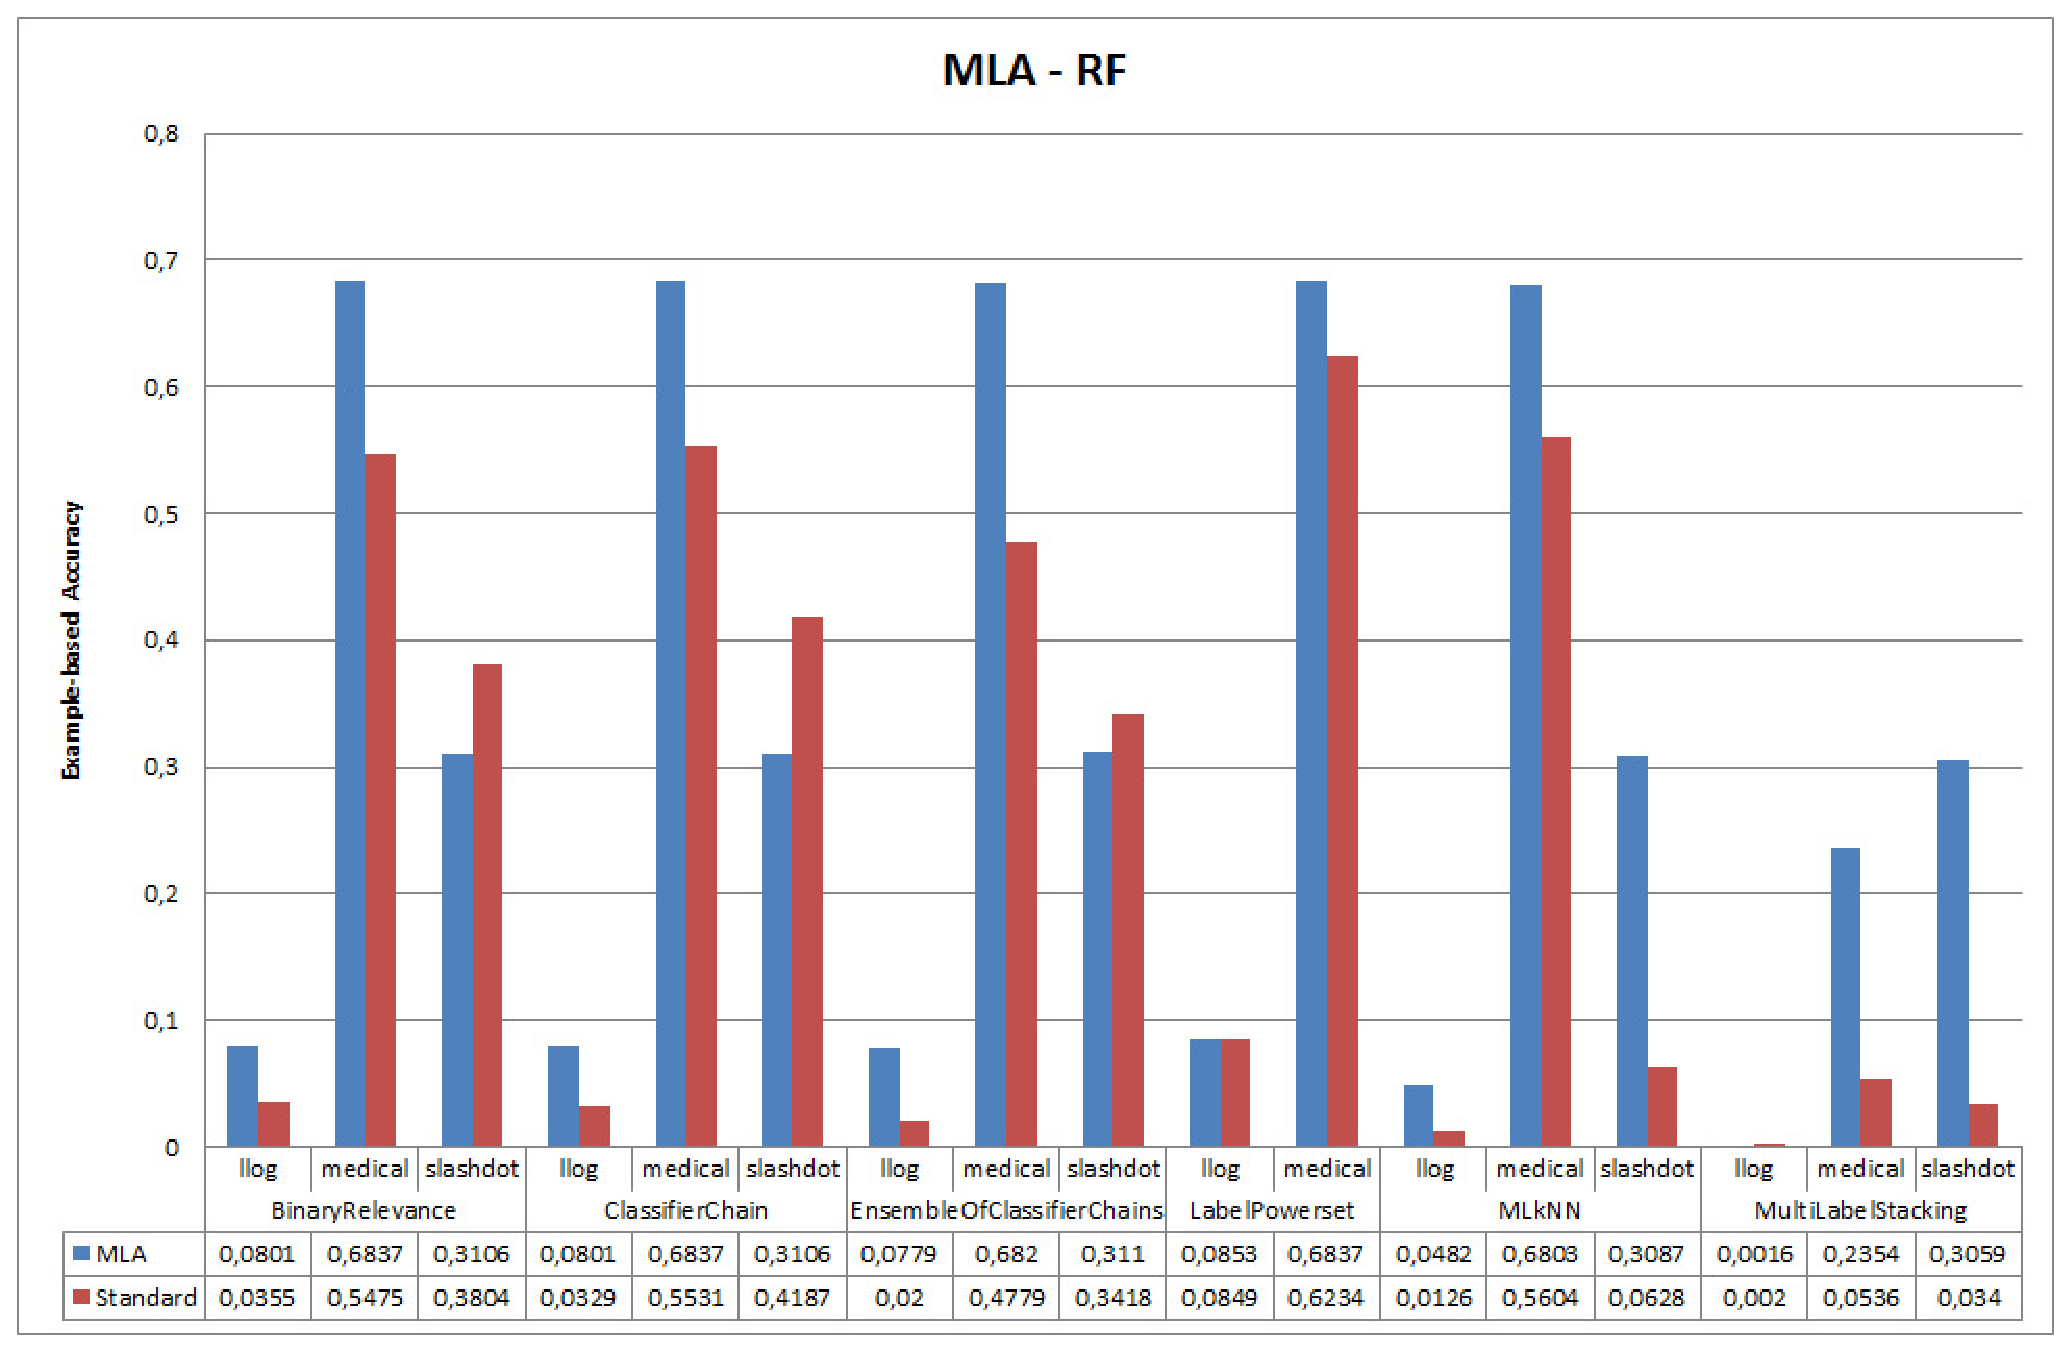
\includegraphics[scale=.3]{figures/mla_results_rf.eps} 
}


\frame{
 {\insertsection} 
		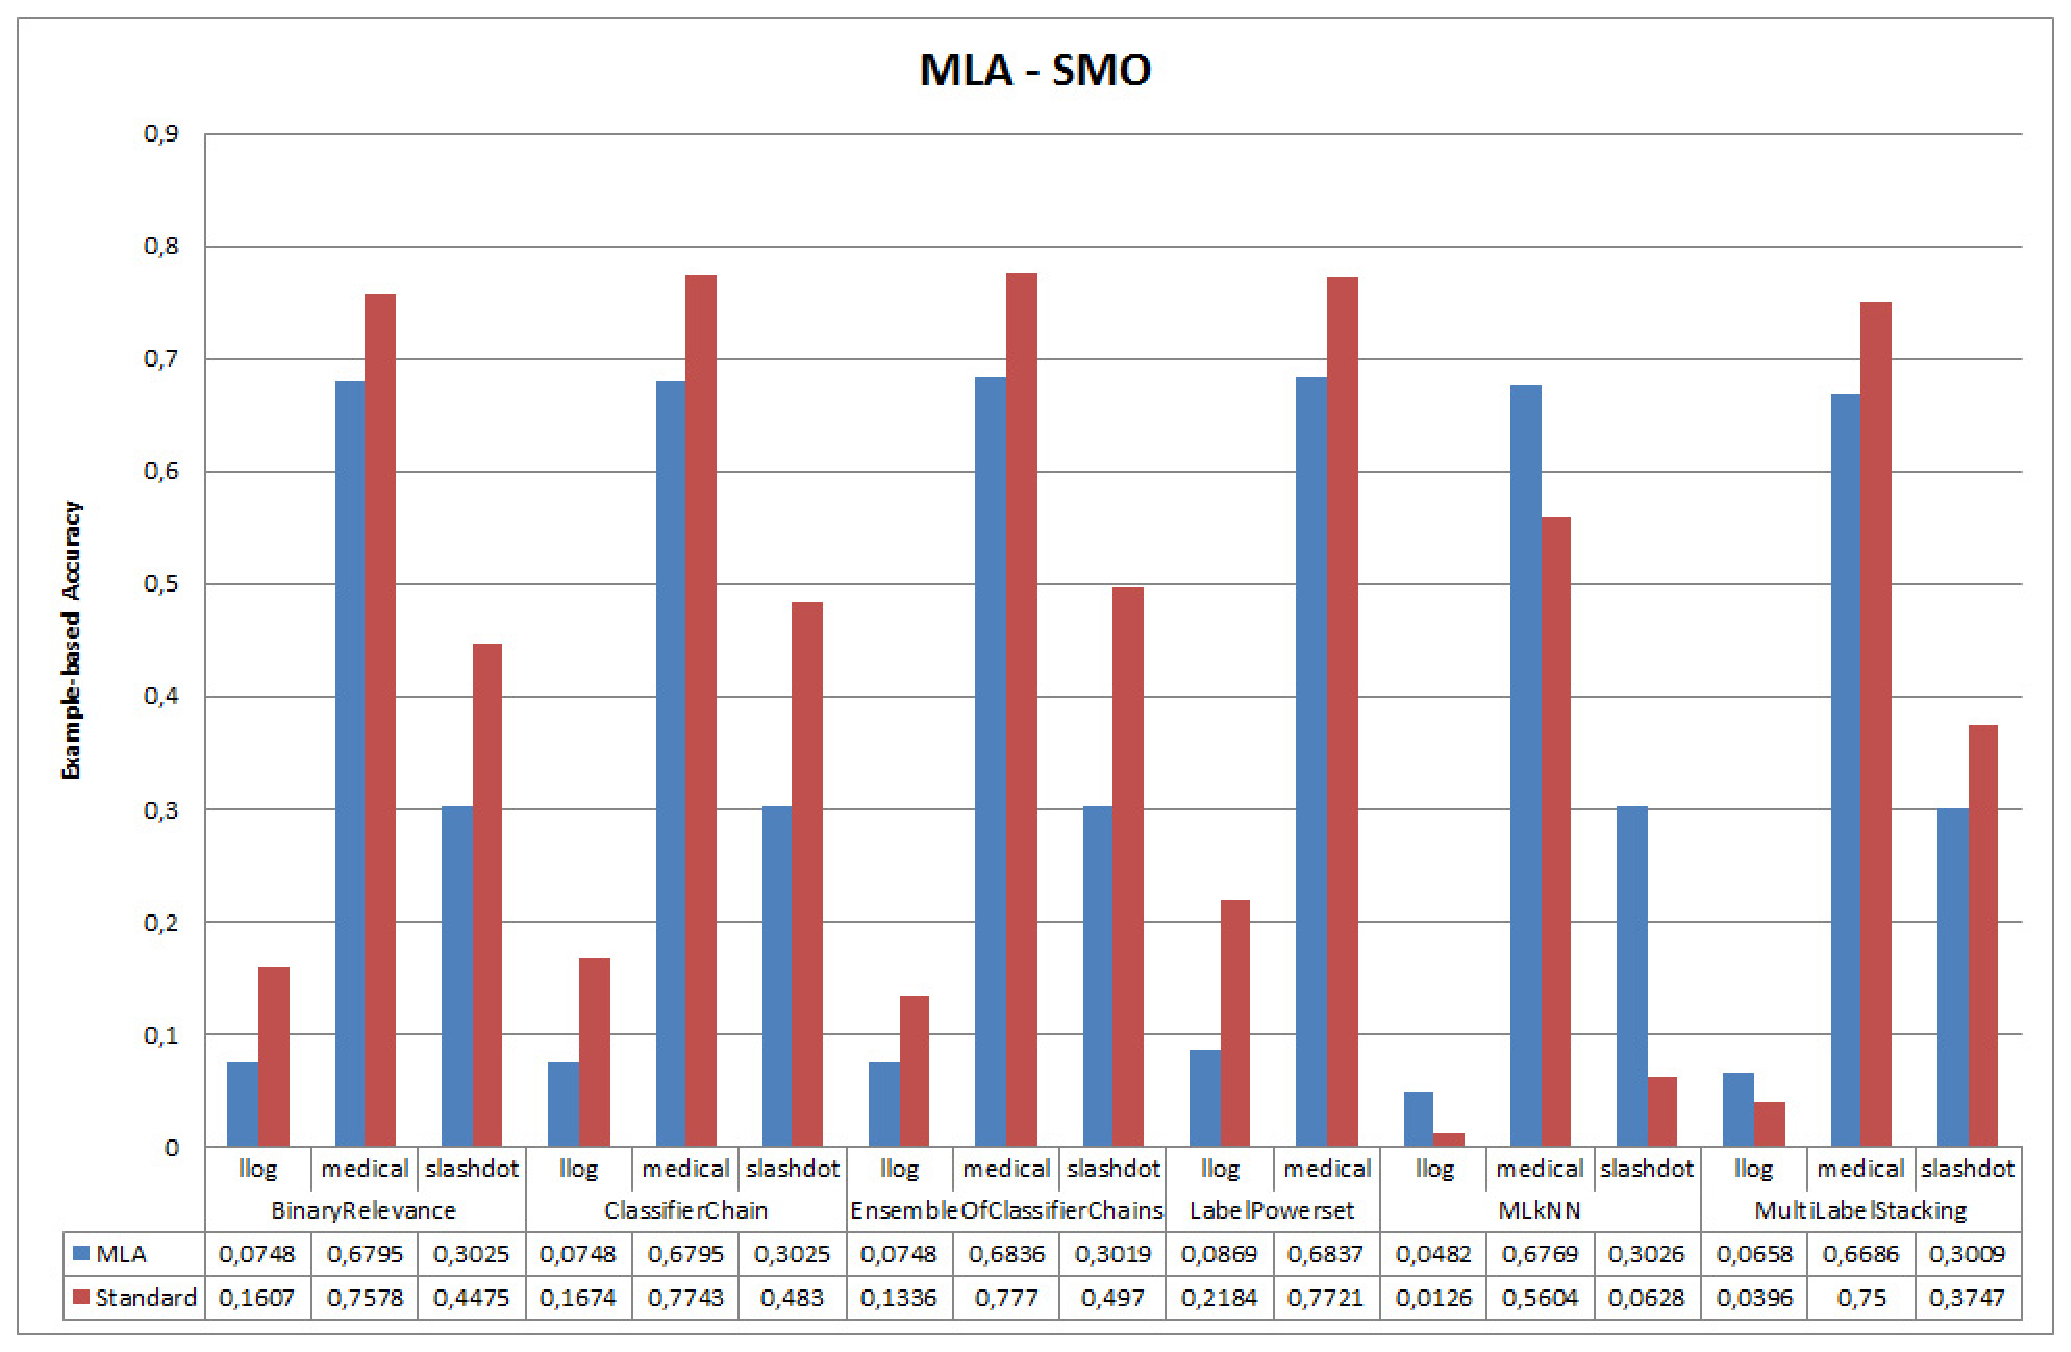
\includegraphics[scale=.3]{figures/mla_results_smo.eps} 
}

\frame{
	{\insertsection}
	example cluster characteristics (\(\varnothing\) over folds)
	\scriptsize {
	\begin{itemize}
		\item llog\\
		\(\varnothing\) number of clusters : 3.8\\
		\(\varnothing\) number of cluster ($> 2$ labels) : 3..6\\
		\(\varnothing\) number of labels per cluster: 19,7	
		\item medical\\
		\(\varnothing\) number of clusters : 13.6\\
		\(\varnothing\) number of cluster ($> 2$ labels) : 4\\
		\(\varnothing\) number of labels per cluster: 3.3	
		\item slashdot\\
		\(\varnothing\) number of clusters : 16.2\\
		\(\varnothing\) number of cluster ($> 2$ labels) : 0.8\\
		\(\varnothing\) number of labels per cluster: 1.4	
	\end{itemize}
	}
}

\end{document}